\documentclass{beamer}
\usetheme{Boadilla}
\usepackage{csquotes}
\usepackage[english]{babel}
\usepackage[utf8]{inputenc}

\usepackage{lipsum}
\usepackage[backend=bibtex,style=authoryear]{biblatex}

\AtBeginBibliography{\small}

\setbeamerfont{bibliography entry author}{size=\tiny}
\setbeamerfont{bibliography entry title}{size=\tiny}
\setbeamerfont{bibliography entry note}{size=\tiny}
\setlength{\biblabelsep}{0.1em}
\usepackage{tabularx}
\usepackage{geometry}
\usepackage{booktabs}


\renewcommand*{\bibfont}{\scriptsize}
\setlength{\columnsep}{1em}
\usepackage{hyperref}

\setbeamertemplate{footline}
{
  \leavevmode%
  \hbox{%
  \begin{beamercolorbox}[wd=.9\paperwidth,ht=2.25ex,dp=1ex,center]{author in head/foot}
    \usebeamerfont{author in head/foot}
    \insertsectionnavigationhorizontal{.7\paperwidth}{}{}
  \end{beamercolorbox}
  \begin{beamercolorbox}[wd=.1\paperwidth,ht=2.25ex,dp=1ex,right]{date in head/foot}
    \usebeamerfont{date in head/foot}
    \insertframenumber{} / \inserttotalframenumber\hspace*{2ex} 
  \end{beamercolorbox}}
  \vskip0pt%
}


\beamertemplatenavigationsymbolsempty

\addbibresource{resources.bib}

\definecolor{LMUGreen}{RGB}{0,45,65}
\definecolor{Black}{RGB}{35,35,35}
\definecolor{White}{RGB}{255,255,255}
\definecolor{Darkgrey}{RGB}{98,100,104}
\definecolor{Middlegrey}{RGB}{192,193,195}
\definecolor{Lightgrey}{RGB}{230,230,231}
\definecolor{Superlightgrey}{RGB}{245,245,245}

\setbeamercolor{item projected}{bg=LMUGreen,fg=White}

\setbeamercolor{section in toc}{fg=Black,bg=White}
\setbeamercolor{alerted text}{fg=LMUGreen}
\setbeamercolor*{palette primary}{fg=LMUGreen,bg=Lightgrey}
\setbeamercolor*{palette secondary}{fg=Blue,bg=Lightgrey}
\setbeamercolor*{palette tertiary}{bg=LMUGreen,fg=White}
\setbeamercolor*{palette quaternary}{fg=LMUGreen,bg=Black}

\setbeamercolor*{sidebar}{fg=LMUGreen,bg=Lightgrey}

\setbeamercolor*{palette sidebar primary}{fg=LMUGreen}
\setbeamercolor*{palette sidebar secondary}{fg=White}
\setbeamercolor*{palette sidebar tertiary}{fg=LMUGreen}
\setbeamercolor*{palette sidebar quaternary}{fg=Lightgrey}

\setbeamercolor{titlelike}{parent=palette primary,fg=LMUGreen}
\setbeamercolor{frametitle}{bg=Lightgrey, fg=LMUGreen}
\setbeamercolor{frametitle right}{bg=Middlegrey}

\setbeamercolor*{separation line}{}
\setbeamercolor*{fine separation line}{}

\setbeamercolor*{bibliography entry author}{fg=LMUGreen}
\setbeamercolor*{bibliography entry note}{fg=LMUGreen!80!white}


\title{Securing IoT Networks}

\author{Student Andrei Vlădescu \\ Professor Dr. Ion Bica}

\institute{UNIVERSITY POLITEHNICA OF BUCHAREST} 

\date{\today}

\begin{document}

\begin{frame}
\titlepage 

\end{frame}

\section{Introduction}

\begin{frame}{Project Description}
    \begin{itemize}
        \item Make IoT more secure
        \item Provide an architecture for deployment
    \end{itemize}
    

\end{frame}

\section{State of the Art}

\begin{frame}{Moving Target Defense}
\begin{itemize}
    \item What is Moving Target Defense? 
    \item How can it help us?
\end{itemize}
    
    \begin{figure}
        \centering
        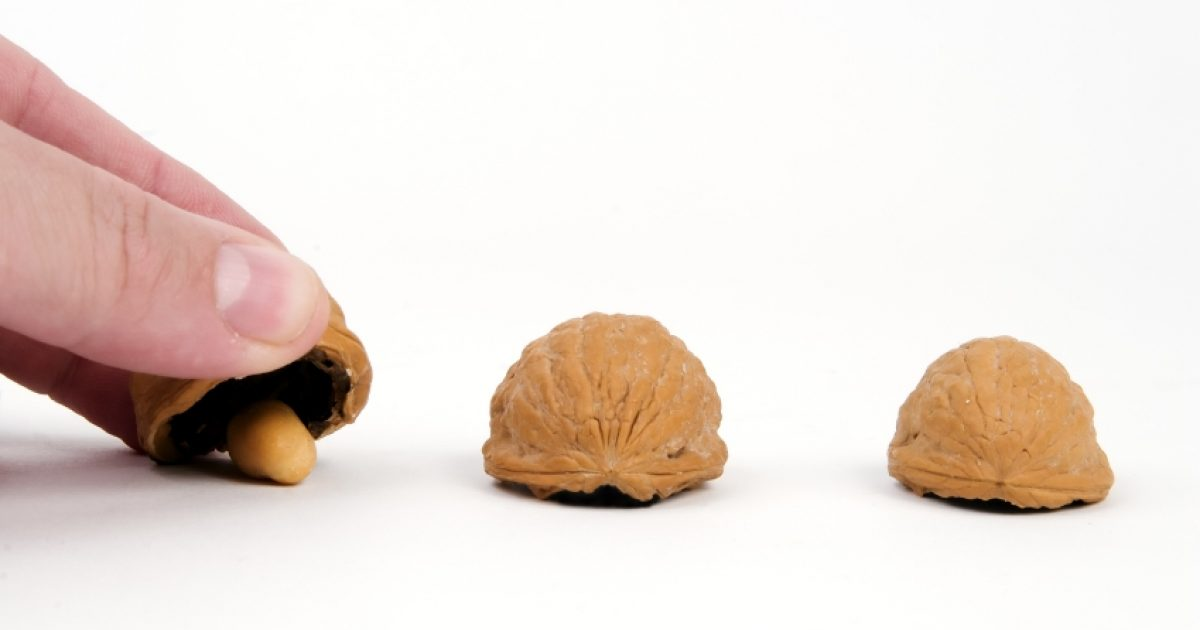
\includegraphics[width=0.55\linewidth]{img/shell.jpg}
        
        \label{fig:enter-label}
    \end{figure}
    %ce este mtd
    %avantaje

\end{frame}


\begin{frame}{State of the Art}
    Key Design Principles:
    \begin{itemize}
        \item What ...to move
        \item When ...to move
        \item How ...to move
    \end{itemize}
\end{frame}

\begin{frame}{State of the Art}
    Already used MTD security mechanisms:
    \begin{itemize}
        \item ASLR %Address Space Layout Randomization
        \item ISR %Instruction Set Randomization
        \item MUTE %Mutable Networks
        \item MSSD %Massive Scale Software Diversity
    \end{itemize}

\end{frame}

\begin{frame}{IoT Security I}

Challenges in securing IoT Networks:
\begin{itemize}
    \item Low power consumption end devices
    \item Limited computing power
    \item Diversity of Devices
\end{itemize}

\end{frame}

\begin{frame}{IoT Security II}
MTD benefits in an IoT Network
\begin{itemize}
    \item Shifting the security challenge to a dedicated device
    \item Implementing honeypots and honeynetworks
    \item Shuffling the physical medium
    \item Dynamically changing encryption algorithms and/or keys
\end{itemize}

\end{frame}

\section{Objectives}

\begin{frame}{Project Objectives I}
Project status:
\begin{itemize}
    \item Researched SoA solutions
    \item Study the possibility of a standardized framework
\end{itemize}
\end{frame}

\begin{frame}{Project Objectives II}
Next semester planning:
\begin{itemize}
    \item Focus on Software Defined Networks (SDN) and external servers
    \item Experiment on a physical network with proposed frameworks
\end{itemize}
\end{frame}

\section{Q&A}

\begin{frame}{Q&A}
  \begin{figure}
    \centering
    
\includegraphics[width=0.75\textwidth]{img/shrek.png}
  \end{figure}
\end{frame}

%-----------------------------------------------
\end{document}